\documentclass{tufte-book}

\hypersetup{colorlinks}% uncomment this line if you prefer colored hyperlinks (e.g., for onscreen viewing)

%%
% Book metadata
\title{Mathematical Methods for Engineers}
\author[CAPT Stu Blair]{United States Naval Academy}
\publisher{Mighty Goat Press}

%%
% If they're installed, use Bergamo and Chantilly from www.fontsite.com.
% They're clones of Bembo and Gill Sans, respectively.
%\IfFileExists{bergamo.sty}{\usepackage[osf]{bergamo}}{}% Bembo
%\IfFileExists{chantill.sty}{\usepackage{chantill}}{}% Gill Sans

%\usepackage{microtype}

%%
% Just some sample text
\usepackage{lipsum}

%%
% For nicely typeset tabular material
\usepackage{tabularx}
\usepackage{booktabs}

%%
% For graphics / images
\usepackage{graphicx}
\setkeys{Gin}{width=\linewidth,totalheight=\textheight,keepaspectratio}
\graphicspath{{graphics/}}

% The fancyvrb package lets us customize the formatting of verbatim
% environments.  We use a slightly smaller font.
\usepackage{fancyvrb}
\fvset{fontsize=\normalsize}

%%
% Prints argument within hanging parentheses (i.e., parentheses that take
% up no horizontal space).  Useful in tabular environments.
\newcommand{\hangp}[1]{\makebox[0pt][r]{(}#1\makebox[0pt][l]{)}}

%%
% Prints an asterisk that takes up no horizontal space.
% Useful in tabular environments.
\newcommand{\hangstar}{\makebox[0pt][l]{*}}

%%
% Prints a trailing space in a smart way.
\usepackage{xspace}

%%%% packages added by Stu

\usepackage{comment}

% fancy enumeration tricks
\usepackage{enumitem}

% have appendices
\usepackage{appendix}

% has sfrac command
\usepackage{xfrac}

% mathtools for over/under brace/bracket among other nifty tools
\usepackage{mathtools}


\usepackage{cancel} % to get oblique strike-through

%\usepackage{minted}
\usepackage{pifont}
\usepackage{color}

\usepackage{listings}
\definecolor{mygreen}{rgb}{0,0.6,0}
\definecolor{mygray}{rgb}{0.5,0.5,0.5}
\definecolor{mymauve}{rgb}{0.58,0,0.82}
\lstset{ %
  backgroundcolor=\color{white},   % choose the background color; you must add \usepackage{color} or \usepackage{xcolor}
  basicstyle=\footnotesize,        % the size of the fonts that are used for the code
  breakatwhitespace=false,         % sets if automatic breaks should only happen at whitespace
  breaklines=true,                 % sets automatic line breaking
  captionpos=b,                    % sets the caption-position to bottom
  commentstyle=\color{mygreen},    % comment style
  deletekeywords={...},            % if you want to delete keywords from the given language
  escapeinside={\%*}{*)},          % if you want to add LaTeX within your code
  extendedchars=true,              % lets you use non-ASCII characters; for 8-bits encodings only, does not work with UTF-8
  frame=single,                    % adds a frame around the code
  inputpath=./matlab_examples/,
  keepspaces=true,                 % keeps spaces in text, useful for keeping indentation of code (possibly needs columns=flexible)
  keywordstyle=\color{blue},       % keyword style
  language=Matlab,                 % the language of the code
  morekeywords={*,...},            % if you want to add more keywords to the set
  numbers=left,                    % where to put the line-numbers; possible values are (none, left, right)
  numbersep=5pt,                   % how far the line-numbers are from the code
  numberstyle=\tiny\color{mygray}, % the style that is used for the line-numbers
  rulecolor=\color{black},         % if not set, the frame-color may be changed on line-breaks within not-black text (e.g. comments (green here))
  showspaces=false,                % show spaces everywhere adding particular underscores; it overrides 'showstringspaces'
  showstringspaces=false,          % underline spaces within strings only
  showtabs=false,                  % show tabs within strings adding particular underscores
  stepnumber=2,                    % the step between two line-numbers. If it's 1, each line will be numbered
  stringstyle=\color{mymauve},     % string literal style
  tabsize=2,                       % sets default tabsize to 2 spaces
  title=\lstname                   % show the filename of files included with \lstinputlisting; also try caption instead of title
}

% example usage for code: \begin{lstlisting}[caption=< caption text >, label=<label>]

%%% end packages added by Stu
%%
% Some shortcuts for Tufte's book titles.  The lowercase commands will
% produce the initials of the book title in italics.  The all-caps commands
% will print out the full title of the book in italics.
\newcommand{\vdqi}{\textit{VDQI}\xspace}
\newcommand{\ei}{\textit{EI}\xspace}
\newcommand{\ve}{\textit{VE}\xspace}
\newcommand{\be}{\textit{BE}\xspace}
\newcommand{\VDQI}{\textit{The Visual Display of Quantitative Information}\xspace}
\newcommand{\EI}{\textit{Envisioning Information}\xspace}
\newcommand{\VE}{\textit{Visual Explanations}\xspace}
\newcommand{\BE}{\textit{Beautiful Evidence}\xspace}

\newcommand{\TL}{Tufte-\LaTeX\xspace}

% Prints the month name (e.g., January) and the year (e.g., 2008)
\newcommand{\monthyear}{%
  \ifcase\month\or January\or February\or March\or April\or May\or June\or
  July\or August\or September\or October\or November\or
  December\fi\space\number\year
}


% Prints an epigraph and speaker in sans serif, all-caps type.
\newcommand{\openepigraph}[2]{%
  %\sffamily\fontsize{14}{16}\selectfont
  \begin{fullwidth}
  \sffamily\large
  \begin{doublespace}
  \noindent\allcaps{#1}\\% epigraph
  \noindent\allcaps{#2}% author
  \end{doublespace}
  \end{fullwidth}
}

% Inserts a blank page
\newcommand{\blankpage}{\newpage\hbox{}\thispagestyle{empty}\newpage}

\usepackage{units}

% Typesets the font size, leading, and measure in the form of 10/12x26 pc.
\newcommand{\measure}[3]{#1/#2$\times$\unit[#3]{pc}}

% Macros for typesetting the documentation
\newcommand{\hlred}[1]{\textcolor{Maroon}{#1}}% prints in red
\newcommand{\hangleft}[1]{\makebox[0pt][r]{#1}}
\newcommand{\hairsp}{\hspace{1pt}}% hair space
\newcommand{\hquad}{\hskip0.5em\relax}% half quad space
\newcommand{\TODO}{\textcolor{red}{\bf TODO!}\xspace}
\newcommand{\na}{\quad--}% used in tables for N/A cells
\providecommand{\XeLaTeX}{X\lower.5ex\hbox{\kern-0.15em\reflectbox{E}}\kern-0.1em\LaTeX}
\newcommand{\tXeLaTeX}{\XeLaTeX\index{XeLaTeX@\protect\XeLaTeX}}
% \index{\texttt{\textbackslash xyz}@\hangleft{\texttt{\textbackslash}}\texttt{xyz}}
\newcommand{\tuftebs}{\symbol{'134}}% a backslash in tt type in OT1/T1
\newcommand{\doccmdnoindex}[2][]{\texttt{\tuftebs#2}}% command name -- adds backslash automatically (and doesn't add cmd to the index)
\newcommand{\doccmddef}[2][]{%
  \hlred{\texttt{\tuftebs#2}}\label{cmd:#2}%
  \ifthenelse{\isempty{#1}}%
    {% add the command to the index
      \index{#2 command@\protect\hangleft{\texttt{\tuftebs}}\texttt{#2}}% command name
    }%
    {% add the command and package to the index
      \index{#2 command@\protect\hangleft{\texttt{\tuftebs}}\texttt{#2} (\texttt{#1} package)}% command name
      \index{#1 package@\texttt{#1} package}\index{packages!#1@\texttt{#1}}% package name
    }%
}% command name -- adds backslash automaticallygit@github.com:stu314159/Nuclear_Plant_Engineering.git
\newcommand{\doccmd}[2][]{%
  \texttt{\tuftebs#2}%
  \ifthenelse{\isempty{#1}}%
    {% add the command to the index
      \index{#2 command@\protect\hangleft{\texttt{\tuftebs}}\texttt{#2}}% command name
    }%
    {% add the command and package to the index
      \index{#2 command@\protect\hangleft{\texttt{\tuftebs}}\texttt{#2} (\texttt{#1} package)}% command name
      \index{#1 package@\texttt{#1} package}\index{packages!#1@\texttt{#1}}% package name
    }%
}% command name -- adds backslash automatically
\newcommand{\docopt}[1]{\ensuremath{\langle}\textrm{\textit{#1}}\ensuremath{\rangle}}% optional command argument
\newcommand{\docarg}[1]{\textrm{\textit{#1}}}% (required) command argument
\newenvironment{docspec}{\begin{quotation}\ttfamily\parskip0pt\parindent0pt\ignorespaces}{\end{quotation}}% command specification environment
\newcommand{\docenv}[1]{\texttt{#1}\index{#1 environment@\texttt{#1} environment}\index{environments!#1@\texttt{#1}}}% environment name
\newcommand{\docenvdef}[1]{\hlred{\texttt{#1}}\label{env:#1}\index{#1 environment@\texttt{#1} environment}\index{environments!#1@\texttt{#1}}}% environment name
\newcommand{\docpkg}[1]{\texttt{#1}\index{#1 package@\texttt{#1} package}\index{packages!#1@\texttt{#1}}}% package name
\newcommand{\doccls}[1]{\texttt{#1}}% document class name
\newcommand{\docclsopt}[1]{\texttt{#1}\index{#1 class option@\texttt{#1} class option}\index{class options!#1@\texttt{#1}}}% document class option name
\newcommand{\docclsoptdef}[1]{\hlred{\texttt{#1}}\label{clsopt:#1}\index{#1 class option@\texttt{#1} class option}\index{class options!#1@\texttt{#1}}}% document class option name defined
\newcommand{\docmsg}[2]{\bigskip\begin{fullwidth}\noindent\ttfamily#1\end{fullwidth}\medskip\par\noindent#2}
\newcommand{\docfilehook}[2]{\texttt{#1}\index{file hooks!#2}\index{#1@\texttt{#1}}}
\newcommand{\doccounter}[1]{\texttt{#1}\index{#1 counter@\texttt{#1} counter}}

% Generates the index
\usepackage{makeidx}
\makeindex

\begin{document}

\begin{fullwidth}
\thispagestyle{empty}
\begin{figure}
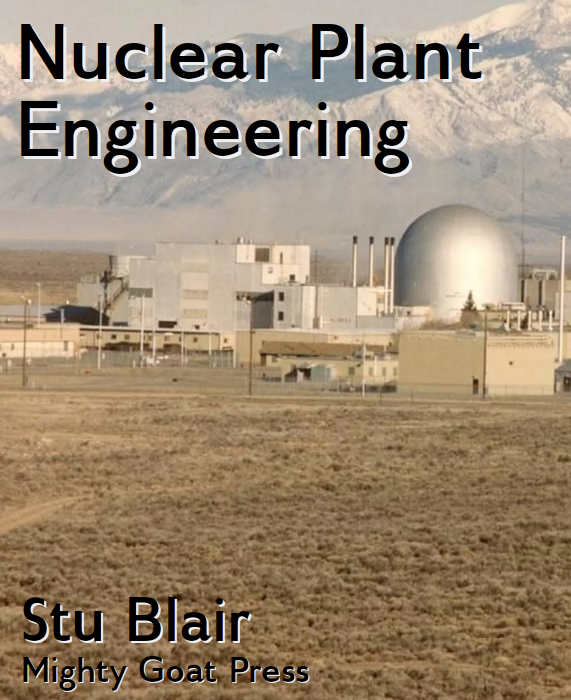
\includegraphics[width=1.5\textwidth]{cover5a.png}
\end{figure}
\end{fullwidth}

% Front matter
\frontmatter

% r.1 blank page
%\blankpage


% v.2 epigraphs
\newpage\thispagestyle{empty}
\vfill
%\openepigraph{
%A good mind may be compared to a vein of precious metal embedded in rock.  If it is to be of value, it %must first be recognized, then laboriously brought forth and carefully worked over.Mathematica - Quantum Physics
%}%{H.G. Rickover}

\vfill
\openepigraph{%
...principles are more important than facts...
}{H.G. Rickover}


\vfill
\openepigraph{%
\ldots one of the prerequisites of originality is the art of forgetting, at the proper moment, what we know. Without this art the mind remains cluttered with ready-made answers and is not forced to ask the proper questions.
}{H.G. Rickover}


% r.3 full title page
\maketitle


% v.4 copyright page
\newpage
\begin{fullwidth}
~\vfill
\thispagestyle{empty}
\setlength{\parindent}{0pt}
\setlength{\parskip}{\baselineskip}
Copyright \copyright\ \the\year\ \thanklessauthor
\par\smallcaps{Published by \thanklesspublisher}

%\par\smallcaps{tufte-latex.github.io/tufte-latex/}
%
%\par Licensed under the Apache License, Version 2.0 (the ``License''); you may not
%use this file except in compliance with the License. You may obtain a copy
%of the License at \url{http://www.apache.org/licenses/LICENSE-2.0}. Unless
%required by applicable law or agreed to in writing, software distributed
%under the License is distributed on an \smallcaps{``AS IS'' BASIS, WITHOUT
%WARRANTIES OR CONDITIONS OF ANY KIND}, either express or implied. See the
%License for the specific language governing permissions and limitations
%under the License.\index{license}

\par\textit{First printing, \monthyear}
\end{fullwidth}

% r.5 contents
\tableofcontents

\listoffigures

\listoftables

% r.7 dedication
%\cleardoublepage
%~\vfill
%\begin{doublespace}
%\noindent\fontsize{18}{22}\selectfont\itshape
%\nohyphenation
%Dedicated to the midshipmen of the United States Naval Academy; the future of our armed services and of %our country.
%\end{doublespace}
%\vfill
%\vfill


% r.9 introduction
\cleardoublepage
\chapter*{Preface}

Preface goes here....



%%
% Start the main matter (normal chapters)
\mainmatter

\part{Introduction and Review}
\chapter{Lecture 1 - Introduction, Definitions and Terminology}
\label{ch:lec1}%<< think of better label and chapter names
\section{Objectives}
The objectives of this lecture are:
\begin{itemize}
\item Provide an overview of course content
\item Define basic terms related to differential equations
\item Provide examples of classification schemes for differential equations
\end{itemize}

\section{Course Introduction}
The basic topics that we will cover include:



\part{Power Series Methods}


%%
% The back matter contains appendices, bibliographies, indices, glossaries, etc.

\part{Back Matter}
\backmatter

\bibliography{Mathematical_Methods_for_Engineers}
\bibliographystyle{plainnat}


\appendix
\appendixpage
\noappendicestocpagenum
\addappheadtotoc



\chapter{Matlab Style Rules}
\begin{enumerate}
\item \textbf{rule:} All scripts will start with the commands: \textbf{clear}, \textbf{clc}, and \textbf{close 'all'}

\textbf{rationale:} No script should depend upon any data visible in the MATLAB workspace when the script starts.  By omitting these commands, residual data within the workspace may hide errors.

\item \textbf{rule:} Your code must be documented with enough details such that a reader unfamiliar with your work will know what you are doing.

\textbf{rationale:} Code documentation is a habit. For more significant projects readers may need help in deciding what the author of the code intended.  For your own code, the most likely reader is you---a few months into the future.

\item \textbf{rule:} Function and variable names must be meaningful and reasonable in length.

\textbf{rationale:} Failing to do either make code harder to read and maintain.

\item \textbf{rule:} All outputs from the code \underline{\textbf{must}} be meaningful; numbers should be formatted, part of a sentence, and include units. Graphs should be readable and axis labels should make sense and include units.

\textbf{rationale:} Code output is a form of communication. It is important that this communication be clear and unambiguous.

\item \textbf{rule:} Do not leave warnings from the Code Analyzer unaddressed.

\textbf{rationale:} Sometimes Code Analyzer warnings can be safely ignored.  Most of the time the warning points to a stylistic error that would be unacceptable in software that you use. Occasionally these warnings are indicative of a hidden error.

\item \textbf{rule:} Use the ``smart indentation tool'' to format the indentation of your code.

\textbf{rationale:} This tool improves code readability. It will also occasionally point out errors that you did not see before.

\item \textbf{rule:} Pre-allocate arrays; if possible initialize with \textbf{NaN} values.

\textbf{rationale:} Pre-allocation improves performance and helps readability. Initialization with \textbf{NaN} helps avoid a range of potential logical errors.

\item \textbf{rule:} Avoid ``magic numbers'' --- i.e. hard-coded constants.

\textbf{rationale:} Constants included in your code tend to hide your program logic. Also, ``magic numbers'' make code maintenance more difficult and error prone.

\item \textbf{rule:} Only write one statement per line.

\textbf{rationale:} Multi-statement-lines hurt code readability in almost all cases.

\item \textbf{rule:} Do not write excessively long lines of code; use the line continuation ``...'' and indentation to spread long expressions over several lines.

\textbf{rationale:} Following this rule improves code readability.
\end{enumerate}


\printindex
\end{document}

